\section{A finite-field tree comparison}\label{sec:tree}

This section isolates the finite-field estimate needed for the auxiliary
primes that will be shared by all leaves in Section~\ref{sec:construction}.
The field size tends to infinity while the tree depth remains
fixed.  In particular, every constant allowed to depend on the depth is
independent of the field, the frequencies, and the other unit parameters
in the tree.

Let $q$ be an odd prime, let $U=\F_q^\times$, and write
$e_q(x)=\exp(2\pi i x/q)$.  For a function on $\F_q$, use the Fourier
normalization
\[
 \widehat f(a)=\frac1q\sum_{x\in\F_q}f(x)e_q(-ax).
\]
For a function on $U$, its Mellin coefficients are
$(q-1)^{-1}\sum_{t\in U}f(t)\overline{\chi(t)}$, where
$\chi\in\widehat U$.  Every multiplicative character, including the
principal character, is extended by zero at zero.  All $L^2$ norms
in this section use probability measure unless a counting sum is
written explicitly.  Suppose throughout
that $g(0)=0$ and $\E_{x\in\F_q}|g(x)|^2\leq1$, and put
\begin{equation}\label{eq:src35}
 \eps_q=\max_{\chi\in\widehat U,\ a\in\F_q}
       \left|\E_{x\in\F_q}g(x)\chi(x)e_q(ax)\right|,
 \qquad \eps_q\longrightarrow0.
\end{equation}
The correlation parameter for $\overline g$ is the same, since conjugation
replaces $(\chi,a)$ by $(\overline\chi,-a)$.  Also $\eps_q\leq1$ by
Cauchy--Schwarz.

\subsection{The diagrams and their elementary density bound}

A diagram of depth $l$ uses a full ordered binary tree with $r=2^l$
leaves.  Its leaf variables $M_i$ take values in $U$.  For a node $n$,
write $M_n$ for the product of the variables at its descendant leaves.
Choose frequencies $s_n\in U$ at every node, a constant $D'\in U$, and
unit constants $C_{n,+},C_{n,-},u_n$ at the internal nodes.  There are
also two current entries $X_{n,+},X_{n,-}$: these are fixed units at the
root and are propagated down the tree as follows.  At an internal node,
set
\begin{equation}\label{eq:src36}
 \begin{split}
 H_{n,\pm}&=X_{n,\pm}C_{n,\pm}M_{n,\pm},\\
 p_n&=\frac{s_{n,+}H_{n,-}-s_{n,-}H_{n,+}}{s_nu_n},\\
 y_n&=\frac{s_n}{D'H_{n,+}H_{n,-}},\\
 y_{n,\pm}&=\frac{s_{n,\pm}}{D'p_nu_nH_{n,\pm}}.
 \end{split}
\end{equation}
The new ordered pair of current entries in child $n,\pm$, when that child
is internal, is $(p_n,X_{n,\pm})$.  The fixed constants are required to
be consistent in the sense that
\[
 H_{n,\pm,+}H_{n,\pm,-}=p_nu_nH_{n,\pm}.
\]
Equivalently, this is the condition
$C_{n,\pm,+}C_{n,\pm,-}=u_nC_{n,\pm}$ on the fixed constants.
It ensures that the formula for a child's argument in its parent's
display agrees with its own formula for $y_n$.

All these operations take place in $\F_q$.  If a reconstructed $p_n$ is
zero, the entire diagram value is defined to be zero, and no division
by that value is performed.  Otherwise define $W$ to be the product of
$g(y_i)$ or $\overline{g(y_i)}$ over the leaves, choosing opposite
conjugations on the two leaves of every bottom sibling pair.  The choices
on different pairs may be arbitrary.  For depth zero set
$y_1=c/M_1$, with a fixed $c\in U$, and take either $g(y_1)$ or its
conjugate.

\begin{lemma}[Tree comparison]\label{lem:tree-comparison}
In a single diagram let the leaf variables be independent uniform
elements of $U$.  Then
\begin{equation}\label{eq:src37}
                       \E|W|^2\leq3^r.
\end{equation}
For two diagrams of the same depth, partition the leaves in each into
$b$ nonempty sets, with the sets in the two diagrams paired.  Give the
two collections of leaf variables the uniform distribution on the
subgroup specified by equality of the products on each paired set.
The diagrams may have different unit parameters and different
conjugation choices.  If $l\geq2$ and $b\leq3r/4$, then under
\eqref{eq:src35}, uniformly in these choices,
\begin{equation}\label{eq:src38}
                         |\E W_1\overline{W_2}|=o_l(1).
\end{equation}
More precisely, the left side is at most
$C_l(\eps_q+q^{-1/4})$ for a constant depending only on $l$.
\end{lemma}

We first prove the density estimate behind \eqref{eq:src37}.  Directly
from \eqref{eq:src36}, on valid points,
\begin{equation}\label{eq:tree-difference-ratio}
 y_n=y_{n,+}-y_{n,-},\qquad
 \frac{y_{n,+}}{y_{n,-}}
       =\frac{s_{n,+}}{s_{n,-}}\frac{H_{n,-}}{H_{n,+}}.
\end{equation}
Expose first the product of all leaf variables.  It is uniform on $U$,
so the root argument is uniform on $U$.  At each successive split,
conditionally on the exposed parent product and all ancestor splits,
$M_{n,+}$ is uniform on $U$ and $M_{n,-}$ is determined by their product.
This follows either by counting the fibers of the product map or by
induction on the two disjoint sets of descendant leaves.  The current
entries are already known at this point.  Consequently the ratio on the
right of \eqref{eq:tree-difference-ratio} is a fixed unit times
$M_{n,+}^{-2}$.  A prescribed valid ordered pair of child arguments
therefore has conditional probability at most $2/(q-1)$.

A specified vector of leaf arguments determines all its intermediate
arguments by taking the indicated differences.  Its probability on the
valid part of the sample space is at most
$2^{r-1}(q-1)^{-r}$.  Thus the joint leaf-argument measure, with invalid
points assigned mass zero, is dominated by $2^{r-1}$ times independent
uniform unit measure.  It follows that
\[
 \E|W|^2
 \leq 2^{r-1}\left(\frac q{q-1}\right)^r
                  \bigl(\E_{x\in\F_q}|g(x)|^2\bigr)^r
 \leq3^r.
\]
Stopping the same exposure at any horizontal level gives the analogous
domination for the arguments at that level.  In particular, the arguments
at the roots of the bottom quartets have joint density bounded by a
constant depending only on $l$ relative to independent uniform unit
arguments.  These are bounds for nonnegative integrals; they place no
pointwise boundedness assumption on $g$.

\subsection{The cycle reduction and the quartet estimates}

We turn to the paired estimate \eqref{eq:src38}. The subgroup distribution
in the statement has the following equivalent description. First choose
independent uniform component totals. In each diagram, independently
given those totals, choose its leaf variables uniformly subject to
the specified product in each component. Every product fiber has the
same cardinality, so this is indeed uniform on the subgroup. Each
diagram separately has independent uniform leaf variables.

In the first diagram make a bipartite multigraph whose vertices are its
$b$ component sets and its $r/4$ bottom quartets, with one edge for each
leaf. It has $r$ edges and at most $r$ vertices, and no isolated
vertices. A forest on nonempty vertex sets has fewer edges than
vertices, so the graph contains a cycle, possibly two parallel edges.
Choose a simple such cycle. On its leaf variables multiply alternately
by $z$ and $z^{-1}$, with $z\in U$. This preserves every component
product and every quartet product. Let $\mathcal P$ denote averaging
over this action, an orthogonal projection in $L^2(U^r)$.

Let $\mathcal T$ be the collection of component totals. The action
preserves their fibers and their uniform measures, so
$\E(W_1\mid\mathcal T)=\E(\mathcal PW_1\mid\mathcal T)$.
Conditional independence of the diagrams, conditional
Cauchy--Schwarz, and \eqref{eq:src37} imply
\begin{equation}\label{eq:tree-projection-reduction}
 |\E W_1\overline{W_2}|
 \leq \|\E(W_1\mid\mathcal T)\|_2\,
       \|\E(W_2\mid\mathcal T)\|_2
 \leq3^{r/2}\|\mathcal PW_1\|_2.
\end{equation}
The last norm uses the first diagram's marginal law of independent
uniform unit leaves; it is not conditioned on the component totals.

Under this law, condition on the products in all bottom quartets.
Ancestor data and ancestor validity are determined by these products.
If an ancestor is invalid the contribution vanishes. Otherwise quartet
interiors are independent uniform product fibers. Each cycle quartet
contains two moving leaves. Fix its two held leaves and use one moving
leaf as a coordinate on $U$; the quartet product determines the other.
Take the Mellin expansion in this coordinate with coefficients
$a_{j,\rho}$. The action scales the coordinate by $z$ or $z^{-1}$,
so projection retains precisely the tuples of indices with
\begin{equation}\label{eq:tree-cycle-relation}
                         \prod_{j=1}^t\rho_j^{\delta_j}=1,
                    \qquad \delta_j\in\{1,-1\},
\end{equation}
where $t$ is the number of quartets on the cycle.

The needed local estimates concern any bottom quartet with its product
and all ancestor data fixed. On valid ancestor data its current entries
and parent argument $y$ are fixed units. Choose two distinct leaves
to move by reciprocal multiplication, preserving their product, and
hold the other two leaves fixed. Use one moving leaf as a coordinate
on $U$; the other is then determined. Write $a_\rho$ for the Mellin
coefficient of the quartet value in this coordinate.

We shall construct nonnegative functions $B_\rho(y)$, depending on $g$
and $q$ but not on the ancestor data or unit parameters, such that
\[
 \E_{\mathrm{held}}|a_\rho|^2\leq B_\rho(y),
\]
and
\begin{equation}\label{eq:src39}
 \sup_\rho\E_{y\in U}B_\rho(y)
       \ll\eps_q^2+q^{-1/2}=o(1),\qquad
 \sum_\rho\E_{y\in U}B_\rho(y)\ll1.
\end{equation}
The held average here is the independent uniform average of the two
held leaf variables, conditional on the quartet product. We shall
also construct a nonnegative $B_0(y)$ of bounded mean that dominates
the full conditional second moment of an untouched quartet. Finitely
many orientations and conjugation choices are possible; adding their
majorants makes all these assertions uniform without affecting their
bounds.

One character in \eqref{eq:tree-cycle-relation} is determined by the
others. We will use the small supremum in \eqref{eq:src39} for that
index, the bounded sum for the remaining indices, and $B_0$ for
quartets off the cycle. The following local calculations establish
these estimates; we then complete the projected norm bound.

\subsection{Bottom-pair autocorrelations}

We next establish the local estimates used in each quartet.  Fix
$\sigma\in\{1,-1\}$ and $g_*\in\{g,\overline g\}$.  For $d\in U$ and
$t\in U\setminus\{1\}$, let
\[
 x=\frac{\sigma dt}{t-1},\qquad z=\frac{\sigma d}{t-1},\qquad
 h(d,t)=g_*(x)\overline{g_*(z)}.
\]
Extend $h$ by zero whenever $d=0$ or $t\in\{0,1\}$.  Thus on valid
arguments $x-z=\sigma d$ and $t=x/z$.
Write
\[
 R_*(d)=\E_{t\in U}|h(d,t)|^2\qquad(d\in U).
\]
The map $(d,t)\mapsto(x,z)$ is a bijection between the valid pairs and
ordered distinct unit pairs, so
\begin{equation}\label{eq:tree-R-mean}
 \E_{d\in U}R_*(d)
 =\frac1{(q-1)^2}\sum_{\substack{x,z\in U\\x\ne z}}
                   |g_*(x)|^2|g_*(z)|^2
 \leq\left(\frac q{q-1}\right)^2.
\end{equation}
For nonzero $d$, the Mellin coefficient of $h(d,\cdot)$ is
\begin{equation}\label{eq:tree-P-definition}
 P_\chi(d)=\frac q{q-1}\E_{x\in\F_q}
       (g_*\overline\chi)(x)
       \overline{(g_*\overline\chi)(x-\sigma d)}.
\end{equation}
Indeed, $t=x/(x-\sigma d)$ gives precisely this coefficient.  Use the
autocorrelation formula \eqref{eq:tree-P-definition} also to define
$P_\chi(0)$; this value is not the Mellin coefficient of the
zero-extended $h(0,\cdot)$.

Let $w_\chi(a)=\widehat P_\chi(a)$ and
$r_\chi=\sum_a w_\chi(a)^2$.  Autocorrelation and additive Fourier
inversion give
\[
 w_\chi(a)=\frac q{q-1}
            |\widehat{g_*\overline\chi}(\sigma a)|^2\geq0,
 \qquad
 P_\chi(0)=\sum_a w_\chi(a)
          =\frac q{q-1}\|g\|_2^2.
\]
In particular,
\begin{equation}\label{eq:src40}
 \begin{gathered}
 \sum_a w_\chi(a)\ll1,\qquad
 \max_{\chi,a}w_\chi(a)\ll\eps_q^2=o(1),\\
 \max_\chi r_\chi\ll\eps_q^2=o(1),\qquad
 \sum_\chi r_\chi\ll1.
 \end{gathered}
\end{equation}
For the last assertion, Mellin Parseval at $d\ne0$ gives
$\sum_\chi|P_\chi(d)|^2=R_*(d)$.  At $d=0$, each of the $q-1$
characters has the same value $q\|g\|_2^2/(q-1)$.  Additive Parseval
and \eqref{eq:tree-R-mean} therefore give the explicit bound
\begin{equation}\label{eq:tree-total-r}
 \sum_\chi r_\chi
 =\frac1q\sum_{d\in\F_q}\sum_\chi|P_\chi(d)|^2
 \leq\frac{2q}{q-1}\leq3.
\end{equation}

We shall repeatedly use the following elementary consequence of Mellin
expansion.  If $f(t)=\sum_\chi c_\chi\chi(t)$ on $U$, $K\in U$, and
$\rho\in\widehat U$, then
\begin{equation}\label{eq:tree-square-pullback}
 \left|\E_{z\in U}f(Kz^{\pm2})\overline{\rho(z)}\right|^2
 \leq2\sum_{\chi^{\pm2}=\rho}|c_\chi|^2.
\end{equation}
To see this, orthogonality makes the coefficient on the left equal to
$\sum_{\chi^{\pm2}=\rho}c_\chi\chi(K)$.  The squaring map on
$\widehat U$ has kernel of size two, so there are at most two terms,
and Cauchy--Schwarz proves the inequality.  Similarly, uniform measure
on any square coset in $U$ is dominated by twice uniform measure on
$U$ for nonnegative integrands.

\subsection{A uniform Mellin estimate}

The following estimate will be applied to the quartet terms in the next
subsection.  For every $\eta\in\widehat U$ and $a\in\F_q$,
\begin{equation}\label{eq:src42}
 \sum_{\chi\in\widehat U}
       |\widehat{P_\chi\chi\eta}(a)|^2
 \leq\frac q{q-1}
       \left(\eps_q^4+\sqrt3\,q^{-1/2}\right)=o(1).
\end{equation}
Here the multiplicative twist sets the value at zero to zero, even if
$\chi\eta$ is principal.

For a proof, expand $h(d,\lambda d)$ in Mellin characters and apply
Parseval in $\lambda\in U$.  The left side of \eqref{eq:src42} equals
\[
 \E_{\lambda\in U}
 \left|\E_{d\in\F_q}h(d,\lambda d)\eta(d)e_q(-ad)\right|^2,
\]
where an argument with $d=0$ or $\lambda d=1$ contributes zero.
In the parametrization $x-z=\sigma d$, $x/z=\lambda d$, solve for
$x$ and $d$ in terms of $z$:
\[
 x=\frac{z^2}{z-\sigma/\lambda},\qquad
 d=\frac{z}{\lambda z-\sigma}.
\]
This is a bijective parametrization of the valid values:
$z\in U\setminus\{\sigma/\lambda\}$ corresponds precisely to
$d\in U\setminus\{1/\lambda\}$.  Setting
$t=\sigma/\lambda$ and $r'=1/z$ gives
$1/x=r'-tr'^2$.  Define
\[
 G(h)=(g_*\eta)(1/h)e_q(-a\sigma/h)\quad(h\in U),\qquad G(0)=0.
\]
The identities $\eta(d)=\overline{\eta(\lambda)}\eta(x/z)$ and
$e_q(-ad)=e_q(-a\sigma x)e_q(a\sigma z)$ show that the inner
coefficient is
\begin{equation}\label{eq:tree-affine-coefficient}
 \overline{\eta(\lambda)}\,TG(t),\qquad
 TF(t)=\frac1q\sum_{r'\in U}\overline{G(r')}
                                      F(r'-r'^2t).
\end{equation}
The zero definition of $G$ encodes exactly the excluded values in this
formula.  Inversion permutes $U$, so
$\|G\|_2\leq1$ and $|\E G|\leq\eps_q$ by
\eqref{eq:src35}.

Here is a direct operator bound for \eqref{eq:tree-affine-coefficient}.
The affine-action estimate is a concrete counterpart of the convolution
bounds developed by Gowers~\cite{Gowers2008}, Babai, Nikolov and
Pyber~\cite{BabaiNikolovPyber2008}, and
Gill~\cite[Theorem~2 and Proposition~1.7]{Gill2016}.
We give the weighted calculation directly in the additive Fourier basis.
Let $U_rF(t)=F(r-r^2t)$, a unitary operator on the probability-normalized
$L^2(\F_q)$.  The map underlying $U_r^*U_s$ is
\[
 t\longmapsto(s/r)^2t+s-s^2/r.
\]
For a prescribed slope, $z=s/r$ has at most two possibilities.  Unless
$z=1$, the translation $r(z-z^2)$ determines $r$ uniquely; $z=1$
gives the identity and forces $r=s$.  Hence every nonidentity affine
map has at most two ordered representations as $U_r^*U_s$.
Write the coefficient array of $T^*T$ on affine maps as $c(a,b)$, with
$a\in U$, $b\in\F_q$, and action $F(t)\mapsto F(at+b)$.
Its identity coefficient is at most $1/q$.  Cauchy--Schwarz on each
fiber of at most two nonidentity representations gives
\begin{equation}\label{eq:tree-affine-coefficient-norm}
 \sum_{a,b}|c(a,b)|^2
 \leq\frac1{q^2}
       +\frac2{q^4}\left(\sum_{r\in U}|G(r)|^2\right)^2
 \leq\frac3{q^2}.
\end{equation}

For completeness, the required affine-action estimate follows from
ordinary additive Parseval.  The functions $e_q(\xi t)$,
$\xi\in U$, form an orthonormal basis of the mean-zero subspace, and
$F(t)\mapsto F(at+b)$ sends the mode $\xi$ to the mode $a\xi$ with
factor $e_q(\xi b)$.  Thus the squared Hilbert--Schmidt norm on this
subspace is
\[
 \sum_{a\in U}\sum_{\xi\in U}
       \left|\sum_b c(a,b)e_q(\xi b)\right|^2
 \leq q\sum_{a,b}|c(a,b)|^2.
\]
Combining with \eqref{eq:tree-affine-coefficient-norm} bounds the
operator norm of $T^*T$ there by $\sqrt3q^{-1/2}$.  Affine actions
preserve the mean-zero subspace and the constants.  If $m_G=\E G$,
then $T1=\overline{m_G}$, so the constant part of $TG$ has squared
norm $|m_G|^4$.  Therefore
\[
 \E_{t\in\F_q}|TG(t)|^2
 \leq\eps_q^4+\sqrt3q^{-1/2}.
\]
Changing the average to $t\in U$, and using that
$\lambda\mapsto\sigma/\lambda$ permutes $U$, proves
\eqref{eq:src42}.

\subsection{Quartet coefficient majorants}

We now construct the majorants in \eqref{eq:src39}. Fix a bottom
quartet with its product and ancestor data as in the cycle reduction.
Let $d,e$ be its two bottom-pair arguments, so $d-e=y$. In either pair,
orient a leaf as free and the other as held.  Its product test is
$h(d,t)$ defined above, with $\sigma$ recording the
orientation and $g_*$ recording the conjugation on the free leaf.

First suppose both moving leaves are in the left pair.  At fixed pair
product, its ratio is a fixed unit times the inverse square of the moving
coordinate.  Equation \eqref{eq:tree-square-pullback} bounds the squared
coefficient by
\[
 2\sum_{\chi^2=\rho^{-1}}|P_\chi(d)|^2
                         \times|\text{right-pair value}|^2.
\]
Interchanging the coordinate convention only inverts $\rho$.
Average the two held variables by exposing first their product and
then their split.  The first exposure makes $d/e$ uniform on a square
coset, and the second makes the right-pair ratio uniform on a square
coset.  Dominate each by twice full unit measure.  Thus a majorant is
a fixed constant times
\begin{equation}\label{eq:tree-same-pair-majorant}
 \frac1{q-1}\sum_{\substack{d,e\in U\\d-e=y}}
       \left(\sum_{\chi^2=\rho^{\pm1}}|P_\chi(d)|^2\right)R_*(e),
\end{equation}
where summing both signs is allowed.  Its mean over $y$ is bounded by
a constant times the product of the means of the two nonnegative
factors: remove the restriction $d\ne e$ to obtain this bound.
Equations \eqref{eq:src40} and \eqref{eq:tree-R-mean} give the two
assertions of \eqref{eq:src39}.  An untouched quartet has the analogous
majorant with $R_L(d)R_R(e)$ in place of the displayed product, and
hence has bounded mean.

It remains to treat one moving leaf in each bottom pair.  The following
diagram records the ordered current entries; the leaf labels underneath
give the corresponding factors $H$ before each bottom reconstruction.
It will explain exactly which held leaves lead to the two formulas below.
\begin{figure}[htbp]
 \centering
 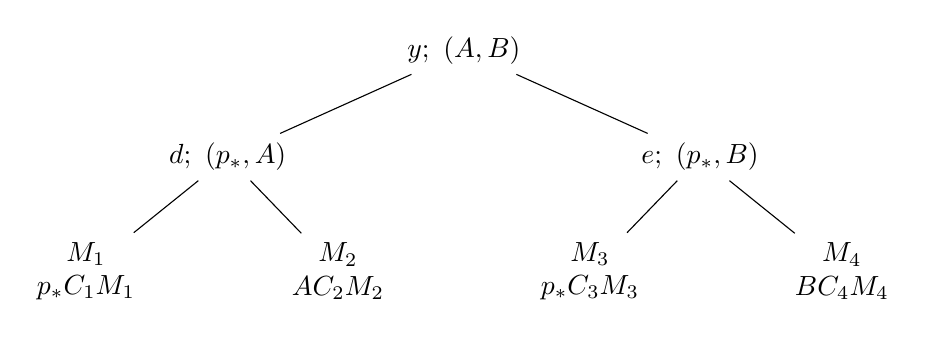
\begin{tikzpicture}
  \node (n) at (0,0) {$y;\ (A,B)$};
  \node (l) at (-3,-1.35) {$d;\ (p_*,A)$};
  \node (r) at (3,-1.35) {$e;\ (p_*,B)$};
  \node[align=center] (ll) at (-4.8,-2.8)
        {$M_1$\\$p_*C_1M_1$};
  \node[align=center] (lr) at (-1.6,-2.8)
        {$M_2$\\$AC_2M_2$};
  \node[align=center] (rl) at (1.6,-2.8)
        {$M_3$\\$p_*C_3M_3$};
  \node[align=center] (rr) at (4.8,-2.8)
        {$M_4$\\$BC_4M_4$};
  \draw (n)--(l) (n)--(r) (l)--(ll) (l)--(lr)
        (r)--(rl) (r)--(rr);
 \end{tikzpicture}
 \caption{A quartet with its ordered current entries.  Here $A,B$ are
 fixed local units, unrelated to the summand sets, and $d-e=y$.
 The shared entry $p_*$ is reconstructed and varies according to
 \eqref{eq:tree-p-square}.  Holding $M_2$
 or $M_4$ uses a residual entry $A$ or $B$; holding $M_1$ or $M_3$
 uses the reconstructed entry $p_*$.}
 \label{fig:tree-quartet}
\end{figure}

Orient the moving leaf as free in each pair.  Division of the formulas
in \eqref{eq:src36} gives
\begin{equation}\label{eq:tree-held-square}
 \frac{t_L}{d}=\text{a fixed unit}\times H_{\mathrm{held},L}^2,
 \qquad
 \frac{t_R}{e}=\text{a fixed unit}\times H_{\mathrm{held},R}^2.
\end{equation}
For example, if the free leaf is the first child of the left pair,
the constant in the first identity is
$D's_{\mathrm{free}}/(s_{\mathrm{held}}s_{\mathrm{pair}})$;
the opposite orientation gives the same form with the two bottom
frequencies interchanged.  At the quartet root, another direct
consequence of \eqref{eq:src36} is
\begin{equation}\label{eq:tree-p-square}
 p_*^2=\frac{s_+s_-}{s_nD'u_n^2}\frac{y}{de}.
\end{equation}
If the held entry in Figure~\ref{fig:tree-quartet} is the residual
$A$ or $B$, \eqref{eq:tree-held-square} therefore has the first of
the following forms; if it is $p_*$, use
\eqref{eq:tree-p-square} to obtain the second:
\begin{equation}\label{eq:tree-friendly-bad}
 t_L=\lambda_Ld\ \text{or}\ \lambda_L/e,
 \qquad
 t_R=\lambda_Re\ \text{or}\ \lambda_R/d.
\end{equation}
Call the first choice on either side friendly and the second bad.
The parameters $\lambda_L,\lambda_R$ are fixed unit multiples of the
squares of the two held leaf variables.  The multiples may depend on
the fixed parent data and on $y$, but not on the held variables.  Since
those variables are independent uniform units, the two parameters
are independent uniform square-coset variables.

For fixed held variables the parent ratio $d/e$ is a fixed unit times
the inverse square of the moving coordinate.  The local value depends
on this ratio, rather than on its square-root choice.  Indeed changing
the moving coordinate to its negative changes $p_*$ to its negative,
while \eqref{eq:tree-friendly-bad} only used its square; the arguments
within either pair are determined by their ratio and their difference.
Apply \eqref{eq:tree-square-pullback}, and then dominate the two
square-coset laws of the held parameters by full independent unit laws.
The latter domination is applied to a nonnegative squared coefficient
and costs at most four.  On changing from $d/e$ to $d-e=y$, the
normalization changes by the bounded factor $q/(q-1)$.  We obtain a
constant times
\begin{equation}\label{eq:src41}
 \sum_{\nu^2=\rho^{\pm1}}
 \E_{\lambda_L,\lambda_R\in U}
 \left|\frac1q\sum_{\substack{d,e\in U\\d-e=y}}
 h_L(d,t_L)h_R(e,t_R)\nu(d/e)\right|^2.
\end{equation}
The sign allows either Mellin convention.  All invalid ratios are
encoded by the zero definitions of the functions $h$; in particular,
the parent ratio $1$ has no valid $(d,e)$ with $d-e=y\ne0$.

To check the sum over $\rho$ in \eqref{eq:src39}, it suffices to sum
over all $\nu$.  For $y\ne0$, the map $t=d/e$ is a bijection from
$U\setminus\{1\}$ to the unit solutions of $d-e=y$, with
$d=yt/(t-1)$ and $e=y/(t-1)$.  Mellin Parseval, followed by the
independent $\lambda_L,\lambda_R$ averages, bounds this sum by a
constant times
\[
 \frac1{q-1}\sum_{\substack{d,e\in U\\d-e=y}}R_L(d)R_R(e).
\]
Its mean over $y\in U$ is bounded by \eqref{eq:tree-R-mean}.

For the small bound at a fixed $\nu$, extend the nonnegative $y$ average
to all of $\F_q$, paying at most $q/(q-1)$.  Expand both $h$ factors
in Mellin characters $\chi,\psi$.  Orthogonality in the independent
parameters separates their squared coefficients.  Additive convolution
Parseval then reduces the bound to
\begin{equation}\label{eq:tree-twisted-convolution}
 \sum_{a,\chi,\psi}
        |\widehat{P_\chi\alpha}(a)|^2
        |\widehat{P_\psi\beta}(-a)|^2.
\end{equation}
Each pair uses its own choice of $\sigma,g_*$ in its $P$.  The twists
are listed explicitly below; all are zero at zero:
\[
\begin{array}{c|cc}
 \text{choices}&\alpha&\beta\\ \hline
 \text{friendly, friendly}&\nu\chi&\overline\nu\psi\\
 \text{friendly, bad}&\nu\chi\overline\psi&\overline\nu\\
 \text{bad, friendly}&\nu&\overline\nu\psi\overline\chi\\
 \text{bad, bad}&\nu\overline\psi&\overline\nu\overline\chi
\end{array}
\]
For example, the left friendly term contributes $\chi(d)$ and the
left bad term contributes $\overline\chi(e)$, which explains all four
rows.  If the left choice is friendly, the second twist is independent
of $\chi$.  Apply \eqref{eq:src42} to the sum over $\chi$, uniformly
in the remaining index and $a$.  The remaining sum is bounded since
additive Parseval gives
\[
 \sum_{\psi,a}|\widehat{P_\psi\beta}(a)|^2
 \leq\sum_\psi\E_{d\in\F_q}|P_\psi(d)|^2\ll1;
\]
here $\beta$ may depend on $\psi$.  This bounds
\eqref{eq:tree-twisted-convolution} by
$O(\eps_q^4+q^{-1/2})$.  The right friendly case is symmetric.

\subsection{The case of two bad choices}

It remains to bound \eqref{eq:tree-twisted-convolution} when
$\alpha=\nu\overline\psi$ and
$\beta=\overline\nu\overline\chi$.  For a nonprincipal character
$\alpha$, the additive Fourier transform of $\alpha$ has constant
modulus $q^{-1/2}$ on nonzero frequencies, and equals zero at zero.
For clarity, the needed Gauss identity follows by substituting
$x\mapsto x/t$ in $\sum_x\alpha(x)e_q(tx)$ for $t\ne0$; its
modulus is $\sqrt q$, because
\[
 \left|\sum_x\alpha(x)e_q(x)\right|^2
 =\sum_{u\in U}\alpha(u)\sum_{z\in U}e_q((u-1)z)
 =(q-1)-\sum_{u\ne1}\alpha(u)=q.
\]
Consequently, with harmless unit factors and a possible reflection
of the frequency,
\begin{equation}\label{eq:tree-Gauss-convolution}
 |\widehat{P_\chi\alpha}(a)|
   =q^{-1/2}\left|\sum_b w_\chi(b)\overline\alpha(a-b)\right|.
\end{equation}

Let $w\geq0$ be any weights of mass $J$ and let $r_w=\sum_b w(b)^2$.
Multiplicative orthogonality yields
\begin{equation}\label{eq:tree-fourth-moment}
 \frac1{q-1}\sum_{\alpha\in\widehat U}\sum_a
       \left|\sum_b w(b)\alpha(a-b)\right|^4
 \leq 2q r_w^2+J^4.
\end{equation}
Indeed, after expansion, a nonzero term requires
\[
 (a-b_1)(a-b_2)=(a-b_3)(a-b_4)\ne0.
\]
When the two unordered pairs of $b$'s agree, their total weight is
at most $2r_w^2$ and there are at most $q$ values of $a$.  Otherwise,
subtracting the two monic quadratics gives a nonzero polynomial of
degree at most one, so there is at most one value of $a$.  The total
weight of all these latter quadruples is at most $J^4$.

The principal character alone contributes
\[
 \frac1{q-1}\sum_a(J-w(a))^4
 \geq\frac{qJ^4-4J^3\sum_aw(a)}{q-1}
 =J^4-\frac{3J^4}{q-1}.
\]
Subtract this contribution in \eqref{eq:tree-fourth-moment} before
applying \eqref{eq:tree-Gauss-convolution}.  Since the masses $J$ of
our $w_\chi$ are uniformly bounded, for each $\chi$ this gives
\[
 \sum_{\alpha\ne1,a}|\widehat{P_\chi\alpha}(a)|^4
 \leq2r_\chi^2+O(q^{-2}).
\]
Summing over $\chi$ and using \eqref{eq:src40}, we obtain
\begin{equation}\label{eq:tree-all-nonprincipal-fourth}
 \sum_{\chi,\alpha\ne1,a}|\widehat{P_\chi\alpha}(a)|^4
 \ll\eps_q^2+q^{-1}.
\end{equation}
When both twists in \eqref{eq:tree-twisted-convolution} are
nonprincipal, Cauchy--Schwarz bounds it by the geometric mean of two
sums of this form.  This is legitimate because at fixed $\nu$ the map
$(\chi,\psi)\mapsto(\chi,\nu\overline\psi)$ is bijective, and the
corresponding assertion holds for the other factor.

We also record the principal cases explicitly.  Because the principal
character is zero at zero, its additive transform is
\begin{equation}\label{eq:tree-principal-correction}
 \widehat{P_\chi\ind_U}(a)=w_\chi(a)-\frac{P_\chi(0)}q.
\end{equation}
Thus its Fourier maximum is $O(\eps_q^2+q^{-1})$, and its squared
Fourier norm is no greater than $r_\chi$ by Parseval on the original
functions.  If $\alpha$ is principal, then $\psi=\nu$ is fixed.
When $\beta$ is nonprincipal,
\eqref{eq:tree-Gauss-convolution} and the bounded mass of
$w_\psi$ bound the other Fourier factor by $O(q^{-1/2})$ uniformly.
Summing the first squared factor over $\chi,a$ costs $O(1)$ by
\eqref{eq:tree-total-r}; this part is $O(q^{-1})$.
The case with the two roles exchanged is identical.  If both twists
are principal, both indices are fixed.  Apply the small Fourier
maximum in \eqref{eq:tree-principal-correction} to one factor and
the bounded squared norm to the other.  This contributes
$O(\eps_q^4+q^{-2})$.

The two-bad case of \eqref{eq:tree-twisted-convolution} is therefore
$O(\eps_q^2+q^{-1})$.  Together with the friendly estimates this
proves the first assertion of \eqref{eq:src39} for
\eqref{eq:src41}.  Adding the finitely many orientation choices and
the same-pair majorants completes the construction of $B_\rho$ and
$B_0$.

\subsection{Completion of the cycle estimate}

Return to the projection in \eqref{eq:tree-projection-reduction},
conditioning again on the products in all bottom quartets.
Orthogonality in
the independent moving coordinates gives a sum of products of
$|a_{j,\rho_j}|^2$, with squared untouched-quartet values as the other
factors.  Average the held variables.  The bounds already proved
dominate this expression by
\[
 \sum_{\prod_j\rho_j^{\delta_j}=1}
             \prod_{j=1}^t B_{\rho_j}(y_j)
             \prod_{j\notin\mathrm{cycle}}B_0(y_j).
\]
The actual joint distribution of quartet arguments on valid ancestor
points is dominated by a constant depending only on $l$ times
independent uniform unit measure, by the horizontal-level density
bound proved above.  Since this last display is nonnegative, we may
use that domination without any pointwise control of $g$.

Put $b_\rho=\E_{y\in U}B_\rho(y)$ and
$b_0=\E_{y\in U}B_0(y)$.  One character in
\eqref{eq:tree-cycle-relation} is determined uniquely by the others.
Consequently
\[
 \|\mathcal PW_1\|_2^2
 \leq C_l\bigl(\sup_\rho b_\rho\bigr)
                 \left(\sum_\rho b_\rho\right)^{t-1}
                 b_0^{r/4-t}
 \ll_l\eps_q^2+q^{-1/2}.
\]
If the cycle consists of two parallel edges, $t=1$ and its sole
character is principal; the same inequality simply uses
$b_1\leq\sup_\rho b_\rho$.  Thus this degenerate cycle requires no
separate structural assumption.  Equation
\eqref{eq:tree-projection-reduction} proves the quantitative statement
of Lemma~\ref{lem:tree-comparison}, and hence \eqref{eq:src38}.

For the later application, the exact transforms $g_p$ in
\eqref{eq:src27} satisfy $g_p(0)=0$ and $\E|g_p|^2=1$ by centering
and additive Parseval.  On the chosen spectator subset their mixed
correlation parameters tend to zero uniformly.  Once independent
unit bulk residues have been obtained in Section~\ref{sec:arithmetic},
Lemma~\ref{lem:tree-comparison} may therefore be applied separately
at every spectator prime.  The zero convention in the diagram retains
the requirement that every reconstructed entry be a unit at that
prime.
